\chapter{Experimentální měření}\label{experiment}

\section{Metodologie}

Pro účely testování jsme využili proces soutěže SMT-COMP\footnote{\url{https://smt-comp.github.io/}}, která od roku 2005 každoročně srovnává nejlepší současné SMT řešiče na velkém množství různorodých testů z~knihovny SMT-LIB. Náš řešič porovnáváme v~kategorii diferenční logiky s~řešiči, které se účastnily soutěže v~roce 2020. Konkrétně to jsou řešiče CVC4, MathSAT\,5, SMTInterpol, veriT, Yices a~z3.

Náš experiment proběhl na 834 testovacích vstupech knihovny SMT-LIB určených pro diferenční logiku. Samotné výpočty probíhaly na počítačích clusteru StarExec\footnote{\url{https://www.starexec.org/}}, iniciativy vzniklé za účelem jednoduššího vytváření, vyhodnocování a~sdílení testů pro různé druhy logických řešičů. Počítače, jež jsou součástí clusteru, obsahují $2.4\rm GHz$ procesor Intel\textregistered\ Xeon\textregistered\ E5-2609, cca.~$250\,\rm GB$ operační paměti a~používají operační systém CentOS verze 7.7 běžící na linuxovém jádře verze 3.10.0

Omezení stanovená pro testy jsme rovněž převzali z~SMT-COMP. Každý test byl spuštěn s~limitem 1200~sekund reálného času, respektive 4800 sekund procesorového času a~s~omezením na $60\,\rm GB$ operační paměti. Výpočet jsme prohlásili za úspěšně dokončený, pokud skončil v~rámci daných limitů a~vrátil korektní odpověď. Jakmile byl některý z~limitů porušen, popřípadě nebyla-li vrácená odpověď korektní, označili jsme test za neúspěšný. Jako primární srovnávací kritérium pak používáme počet úspěšně vyřešených testů a~sekundárním kritériem je celkový čas výpočtů (výpočty ukončené z~důvodu vypršení času jsou započítány s~časem $1200\,\rm s$).

\section{Výsledky}

Přehled výsledků nahlédneme v~tabulce níže, následující strana ilustruje srovnání řešičů s~OpenSMT na úspěšných testech (osy mají logaritmické měřítko a~označují reálný čas výpočtu v~sekundách). Dodejme ještě, že žádný z~testů neskončil nesprávným ohodnocením a~všechny testy se vešly do paměťového limitu --- veškerá předčasná ukončení byla způsobena překročením omezení pro reálný čas.

\begin{table}[h]
	\centering
	\begin{tabular}{l@{\hspace{1cm}} D{.}{,}{3.0} D{.}{,}{6.1} D{.}{,}{3.0} D{.}{,}{3.0} D{.}{,}{3.0}}
		\toprule  
		& \mc{\textbf{Úspěšně}} & \mc{\textbf{Reálný}} & \mc{\textbf{Vyřešeno}} & \mc{\textbf{Vyřešeno}} & \mc{} \\
		\pulrad{\textbf{Řešič}} &\mc{\textbf{vyřešeno}} & \mc{\textbf{čas}} & \mc{\textbf{SAT}} & \mc{\textbf{UNSAT}} & \mc{\pulrad{\textbf{Timeout}}}\\
		\midrule
		Yices & 740 & 128683.6 & 484 & 256 & 94 \\
		z3$^n$ & 727 & 124296.1 & 485 & 242 & 82 \\
		CVC4 & 682 & 231953.6 & 425 & 257 & 152\\
		\textbf{OpenSMT} & 661 & 260896.8 & 412 & 249 & 173 \\
		veriT & 621 & 308952.9 & 372 & 249 & 213\\
		MathSAT\,5$^n$ & 585 & 337559.4 & 341 & 244 & 249\\
		SMTInterpol & 546 & 396759.1 & 313 & 233 & 288\\
		\bottomrule
		\multicolumn{6}{l}{\footnotesize \textit{Pozn:}$^n$ 
		Řešič byl zařazen do měření SMT-COMP, ale nebyl oficiálně registrován jako soutěžící. }
	\end{tabular}
	%\caption{Srovnání SMT řešičů}
\end{table}

\begin{figure}
	\centering
		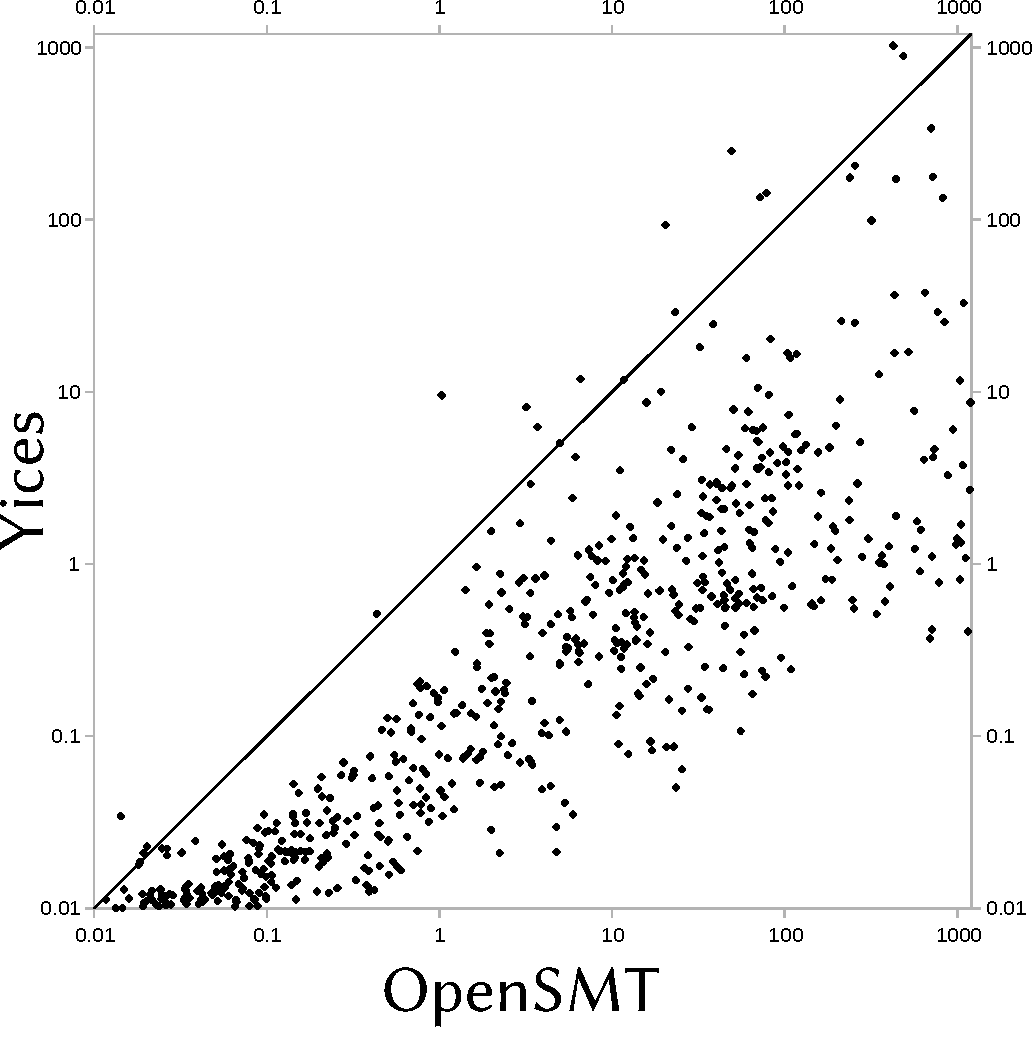
\includegraphics[width=0.49\linewidth]{comp_yices}
		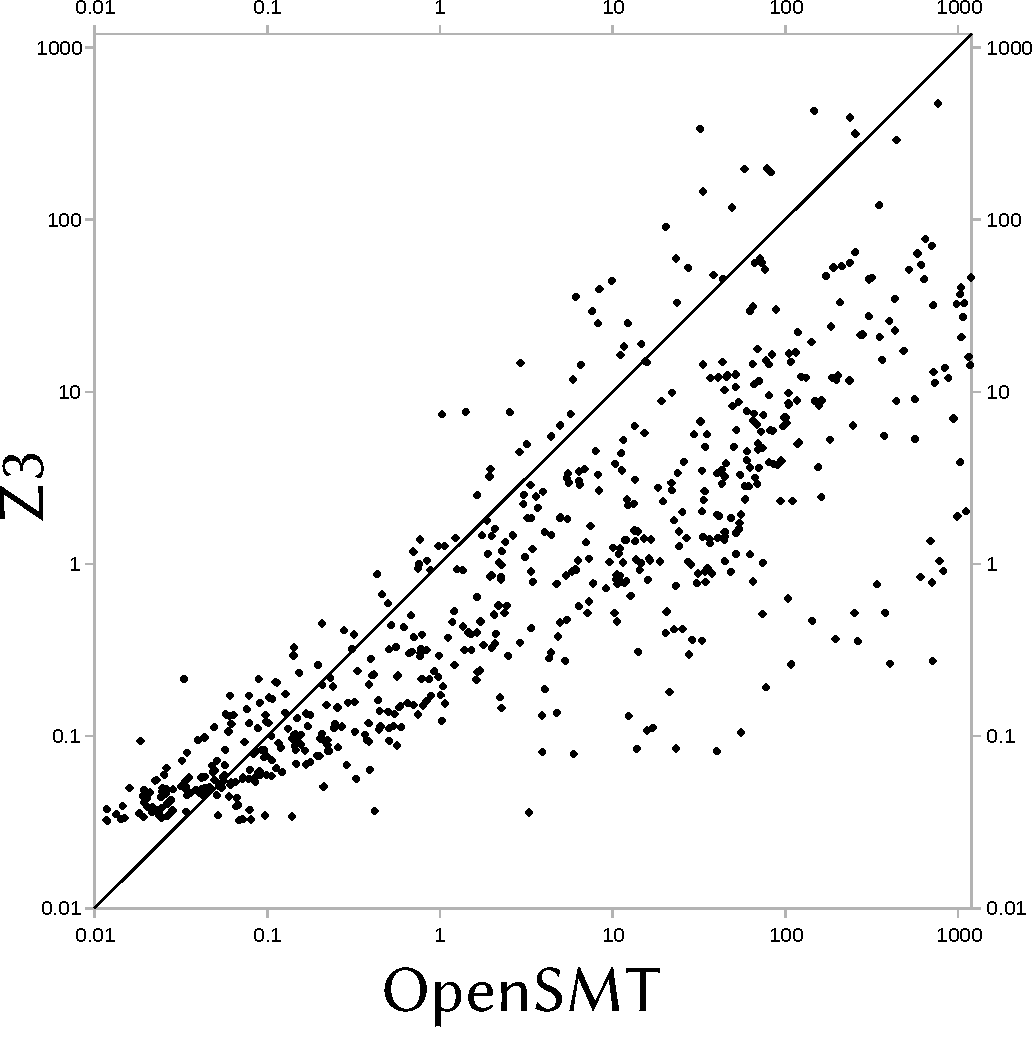
\includegraphics[width=0.49\linewidth]{comp_z3}\\
		\vspace{5px}
		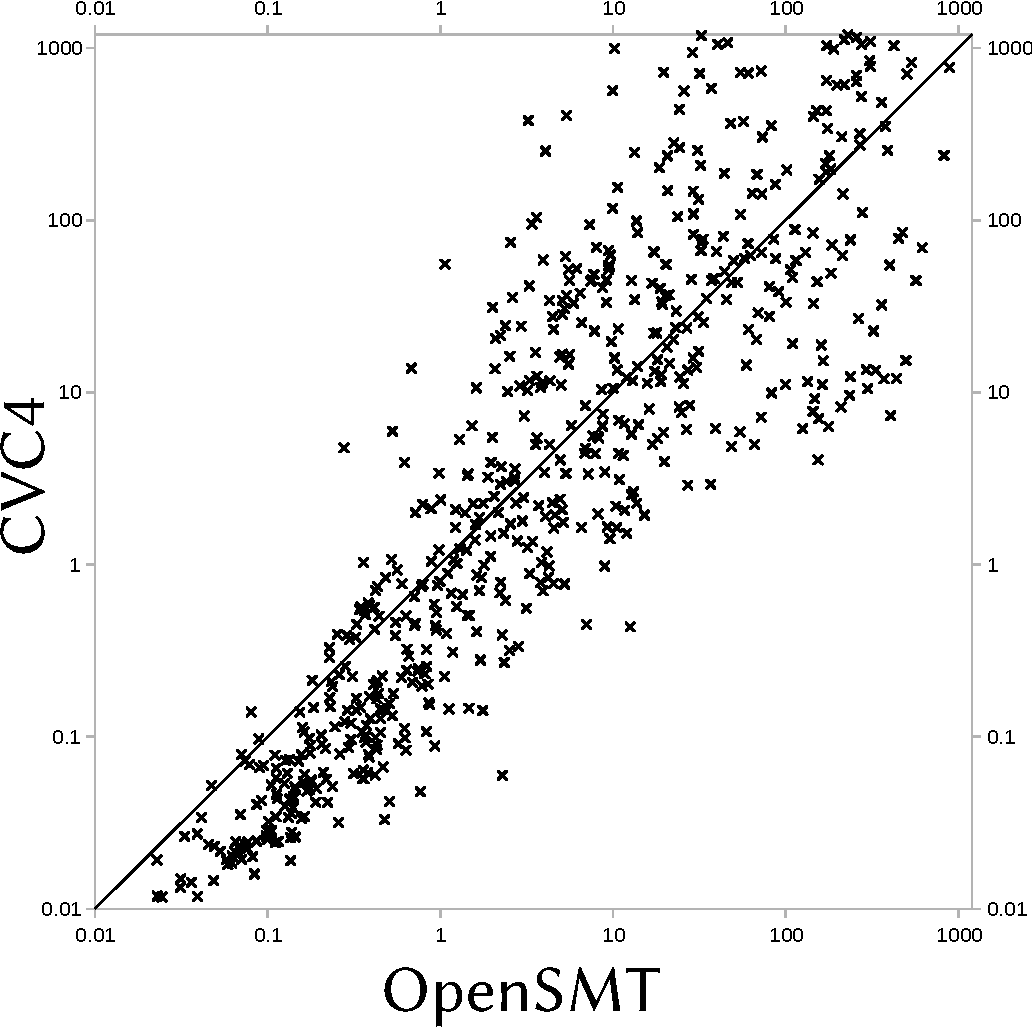
\includegraphics[width=0.49\linewidth]{comp_cvc}
		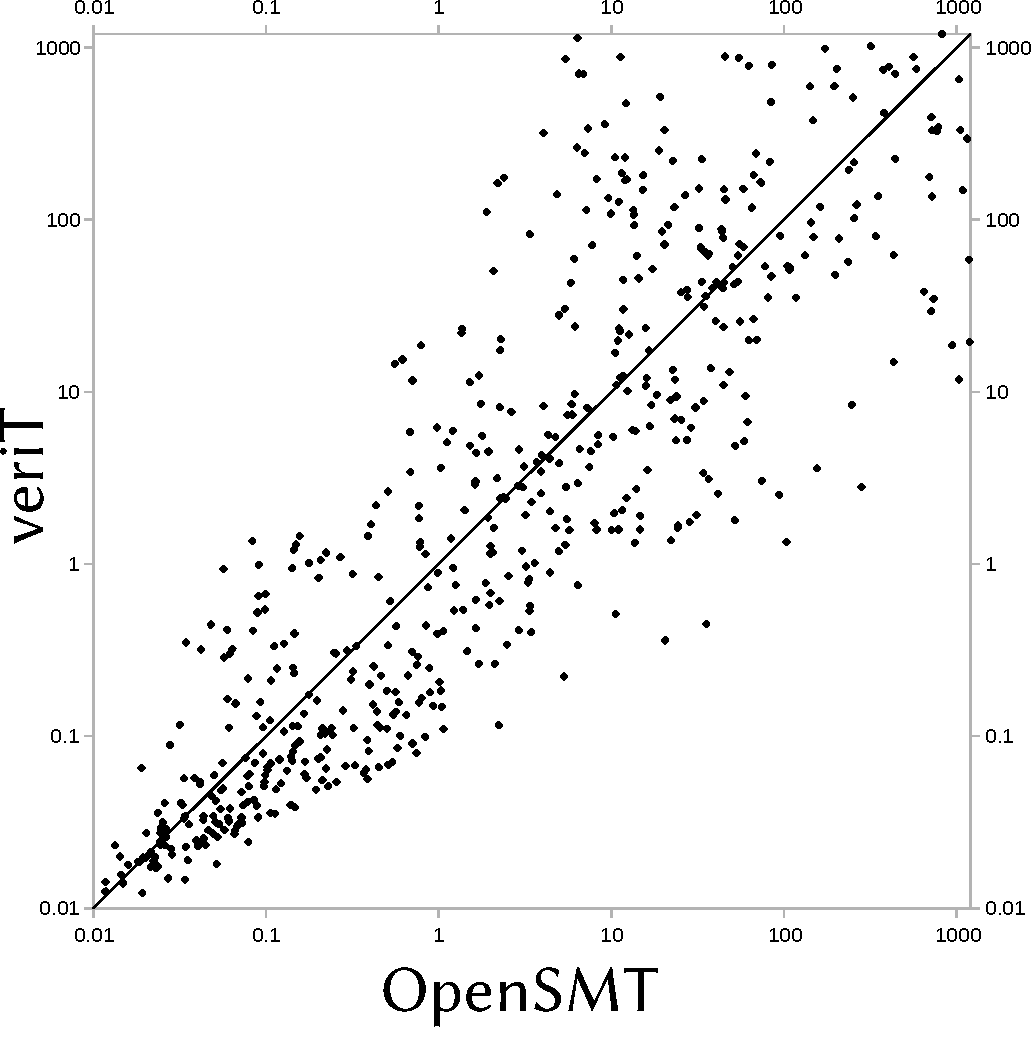
\includegraphics[width=0.49\linewidth]{comp_verit}\\
		\vspace{5px}
		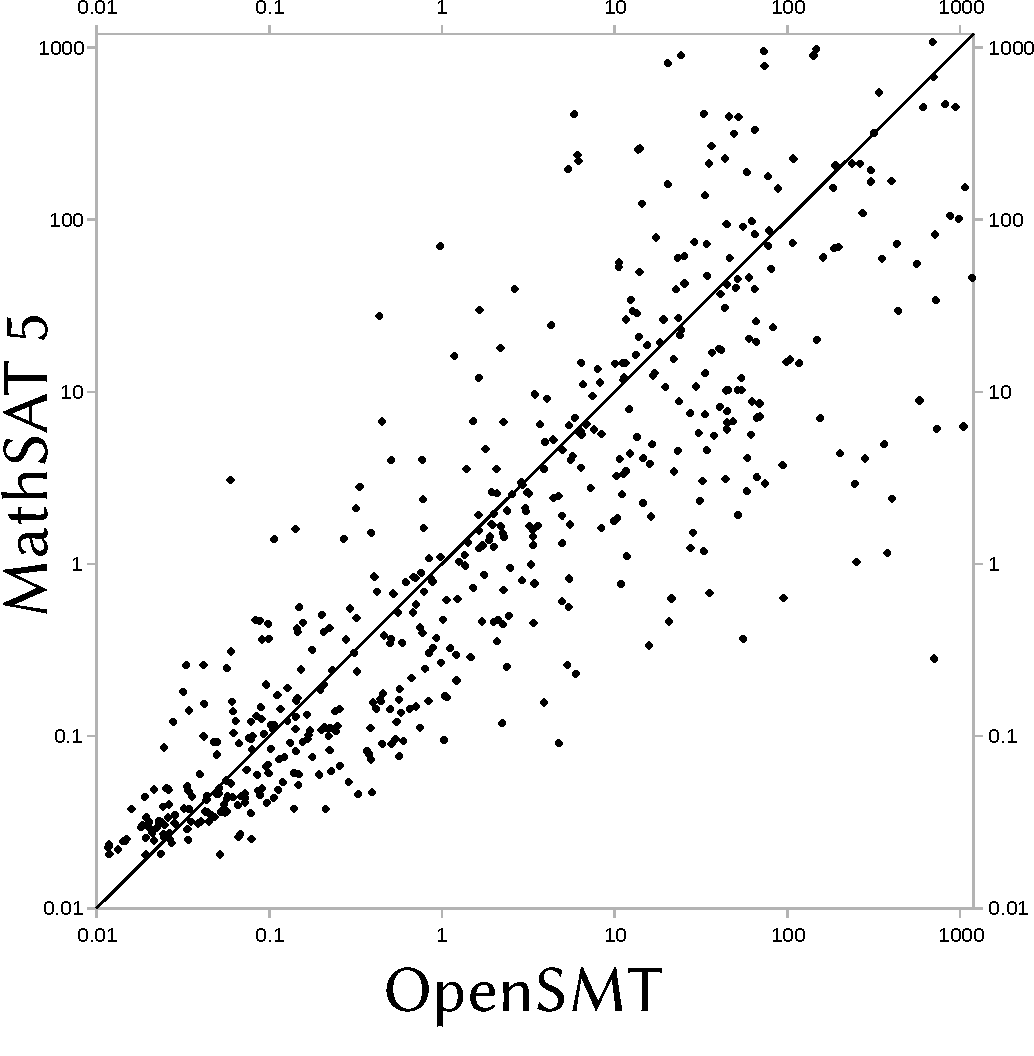
\includegraphics[width=0.49\linewidth]{comp_mathsat}
		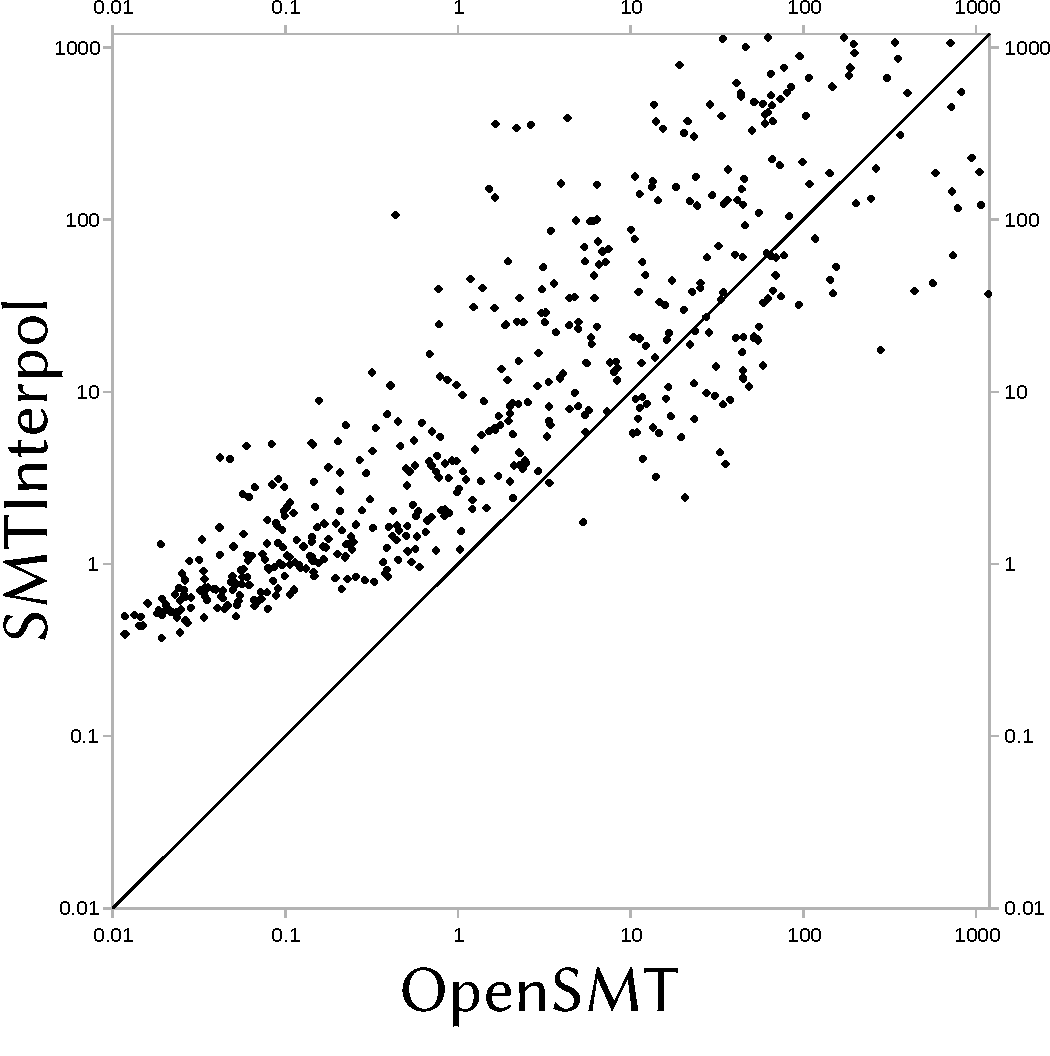
\includegraphics[width=0.49\linewidth]{comp_smti}
		\caption{Srovnání OpenSMT s~ostatními SMT řešiči na vyřešených testech}
\end{figure}

\section{Srovnání}

Jak vidíme, OpenSMT se zařadilo do průměru soutěžících --- v~letošním ročníku soutěže SMT-COMP by skončil na čtvrtém místě. Nemůže se zatím rovnat s~nejlepšími řešiči Yices a~z3, které úspěšně vyřešily o~79, resp. o~62 testů více. Se všemi ostatními však má minimálně srovnatelné hodnocení. V~porovnání s~CVC4 jsme dosáhli takřka $97\,\%$ vyřešených testů a~byli jsme dokonce znatelně úspěšnější než řešiče veriT, SMTInterpol a~MathSAT.

Fakt, že náš řešič ve všech 682 vyřešených testech vrátil správné řešení, navíc můžeme brát jako relativně silný důkaz jeho korektnosti. Tyto výsledky tedy považujeme za úspěch jak frameworku OpenSMT, tak naší implementace řešiče diferenční logiky.
